 \subsection{Project Timeline}
\label{actual-project-timeline}

 For a better visualization of the comparison between the initial project timeline and the actual one, a comparative table is displayed in Table \ref{table:comparison-of-planned-and-actual-effort-per-task}. Beyond that, a new Gantt diagram representing the actual execution progress is also created and corresponds to Figure \ref{fig:gantt2}. 

 
 \newpage
 
    \vspace{10pt}
    %Table of personnel cost breakdown by task and role
    \pagestyle{fancy}
    \scriptsize
    \setlength{\tabcolsep}{2pt}
    \setlength{\arrayrulewidth}{0.1pt}
    \renewcommand{\arraystretch}{1.15}
    \setlength{\LTpre}{0pt}
    \setlength{\LTpost}{0pt}
    \setlength{\LTleft}{0cm} 
    \setlength{\LTright}{0cm}
    \begin{longtable}{l p{10cm} >{\raggedleft\arraybackslash}p{1.5cm} >{\raggedleft\arraybackslash}p{1.5cm} >{\raggedleft\arraybackslash}p{1.5cm}}    \rowcolor{gray!45}
    \textbf{ID} & \textbf{Name} & \textbf{Planned Effort (h)} & \textbf{Actual Effort (h)} & \textbf{Effort Variance (\%)} \\
    \addlinespace[0pt]
    \endfirsthead

    \noalign{\vskip -15pt}
    \multicolumn{5}{l}{\textit{(Continued from previous page)}} \\
    \rowcolor{gray!45}
    \textbf{ID} & \textbf{Name} & \textbf{Planned Effort (h)} & \textbf{Actual Effort (h)} & \textbf{Effort Variance (\%)} \\
    \addlinespace[0pt]
    \endhead
    
    \hline 
    \multicolumn{5}{r}{\textit{(Continued on next page)}} \\
    \noalign{\vskip -12pt} 
    \endfoot

    \hline 
    \addlinespace[0pt] 
    \rowcolor{gray!45} 
    \textbf{Total} & & \textbf{513} & \textbf{542.5} & \textbf{5.75} \\
    \caption[Comparison of planned and actual effort per task, including effort variance]
    {Comparison of planned and actual effort per task, including effort variance. [Own creation]} 
    \vspace{-1em}
    \label{table:comparison-of-planned-and-actual-effort-per-task} 
    \endlastfoot

    \rowcolor{gray!20}
    \textbf{PS} & \textbf{Project Starting} & \textbf{50.00} & \textbf{50.00} & \textbf{0.00} \\ 
    \rowcolor{gray!05}
    PS1 & Context and Scope & 20.00 & 20.00 & 0.00 \\
    \rowcolor{gray!05}
    PS2 & Temporal Planning & 10.00 & 10.00 & 0.00 \\ 
    \rowcolor{gray!05}
    PS3 & Budget and Sustainability & 10.00 & 10.00 & 0.00 \\ 
    \rowcolor{gray!05}
    PS4 & Initial Documentation & 10.00 & 10.00 & 0.00 \\ 

    \rowcolor{gray!20}
    \textbf{PM} & \textbf{Project Management} & \textbf{46.50} & \textbf{46.50} & \textbf{0.00} \\ 
    \rowcolor{gray!05}
    PM1 & Product Owner Meetings & 30.50 & 30.50 & 0.00 \\ 
    \rowcolor{gray!05}
    PM2 & Thesis Director Review Meetings & 8.00 & 8.00 & 0.00 \\ 
    \rowcolor{gray!05}
    PM3 & Product Backlog Update & 8.00 & 8.00 & 0.00 \\ 

    \rowcolor{gray!20}
    \textbf{FPD} & \textbf{Final Product Delivery} & \textbf{56.50} & \textbf{106.00} & \textbf{87.61} \\ 
    \rowcolor{gray!05}
    FPD1 & User Manual Documentation & 2.00 & 2.00 & 0.00 \\ 
    \rowcolor{gray!05}
    FPD2 & Final Thesis Documentation & 30.50 & 80.00 & 162.30 \\ 
    \rowcolor{gray!05}
    FPD3 & Final Demonstration Video & 4.00 & 4.00 & 0.00 \\ 
    \rowcolor{gray!05}
    FPD4 & Bachelor’s Thesis Defense & 20.00 & 20.00 & 0.00 \\ 

    \rowcolor{gray!20}
    \textbf{DT} & \textbf{Design} & \textbf{16.00} & \textbf{16.00} & \textbf{0.00} \\ 
    \rowcolor{gray!05}
    DT1 & Use Case Diagram & 2.00 & 2.00 & 0.00 \\ 
    \rowcolor{gray!05}
    DT2 & Conceptual Model Diagram & 4.00 & 4.00 & 0.00 \\ 
    \rowcolor{gray!05}
    DT3 & Technology Stack Decision & 2.00 & 2.00 & 0.00 \\ 
    \rowcolor{gray!05}
    DT4 & Logic and Physic Architecture Design & 4.00 & 4.00 & 0.00 \\ 
    \rowcolor{gray!05}
    DT5 & UI Mockups Design & 2.00 & 2.00 & 0.00 \\ 
    \rowcolor{gray!05}
    DT6 & Security Design & 2.00 & 2.00 & 0.00 \\ 

    \rowcolor{gray!20}
    \textbf{Dev} & \textbf{Development} & \textbf{86.00} & \textbf{78.00} & \textbf{-9.30} \\ 
    \rowcolor{gray!05}
    Dev0 & Self-learning and study of unfamiliar technologies & 8.00 & 8.00 & 0.00 \\ 
    \rowcolor{gray!05}
    Dev1 & Environment Configuration & 2.00 & 2.00 & 0.00 \\ 
    \rowcolor{gray!05}
    Dev2 & Product Deployment & 8.00 & 20.00 & 150.00 \\ 
    \rowcolor{gray!05}
    Dev3 & CI/CD Pipeline Implementation & 20.00 & 28.00 & 40.00 \\ 
    \rowcolor{gray!05}
    Dev4 & Logging and Monitoring & 8.00 & 0.00 & -100.00 \\ 
    \rowcolor{gray!05}
    Dev6 & Git Repository Documentation & 40.00 & 20.00 & -50.00 \\ 

    \rowcolor{gray!20}
    \multicolumn{2}{l}{\textbf{Frontend and Backend Development}} & 128.00 & 128.00 & 0.00 \\ 

    \rowcolor{gray!10}
    \textbf{ER} & \textbf{Expense and Report Development} & \textbf{64.00} & \textbf{64.00} & \textbf{0.00} \\ 
    \rowcolor{gray!05}
    ER1 & Expense Uploads & 16.00 & 16.00 & 0.00 \\ 
    \rowcolor{gray!05}
    ER2 & Uploaded Expenses Real-time Dashboard & 4.00 & 4.00 & 0.00 \\ 
    \rowcolor{gray!05}
    ER3 & AI-Extracted Expense Data Review and Correction & 20.00 & 20.00 & 0.00 \\ 
    \rowcolor{gray!05}
    ER4 & Uploaded Expenses Deletion & 4.00 & 4.00 & 0.00 \\ 
    \rowcolor{gray!05}
    ER5 & Expense Reports View, Creation, Edit, Submission, and Deletion & 20.00 & 20.00 & 0.00 \\ 

    \rowcolor{gray!10}
    \textbf{UA} & \textbf{User Access Development} & \textbf{64.00} & \textbf{54.00} & \textbf{-15.63} \\  
    \rowcolor{gray!05}
    UA1 & Company Email User Authentication & 8.00 & 8.00 & 0.00 \\
    \rowcolor{gray!05}  
    UA2 & Role-based User Access & 16.00 & 16.00 & 0.00 \\ 
    \rowcolor{gray!05}
    UA3 & Submitted Report Approval and Rejection & 8.00 & 16.00 & 100.00 \\ 
    \rowcolor{gray!05}
    UA4 & Employee Spending Limit Configuration & 8.00 & 0.00 & -100.00 \\ 
    \rowcolor{gray!05}
    UA5 & Report History Categorization by Status and User Role & 4.00 & 4.00 & 0.00 \\ 
    \rowcolor{gray!05}
    UA6 & Email Notification Service Integration & 20.00 & 10.00 & -50.00 \\ 

    \rowcolor{gray!20}
    \textbf{BD} & \textbf{Backend Development} & \textbf{120.00} & \textbf{120.00} & \textbf{0.00} \\
    \rowcolor{gray!05}
    BD1 & RESTful API Backend Logic Implementation & 20.00 & 20.00 & 0.00 \\ 
    \rowcolor{gray!05}
    BD2 & Azure SQL Database Integration and Manipulation & 20.00 & 40.00 & 100.00 \\ 
    \rowcolor{gray!05}
    BD3 & Azure Blob Storage Integration & 8.00 & 8.00 & 0.00 \\ 
    \rowcolor{gray!05}
    BD4 & Microsoft Document Intelligence AI Model Integration & 20.00 & 10.00 & -50.00 \\
    \rowcolor{gray!05}
    BD5 & Automated AI-driven Data Extraction Pipeline & 20.00 & 10.00 & -50.00 \\ 
    \rowcolor{gray!05}
    BD6 & Azure SignalR Real-time Notification Service Integration & 16.00 & 16.00 & 0.00 \\ 
    \rowcolor{gray!05}
    BD7 & Microsoft Entra ID User Authentication Integration & 16.00 & 16.00 & 0.00 \\ 

    \rowcolor{gray!20}
    \textbf{FD} & \textbf{Frontend Development} & \textbf{10.00} & \textbf{8.00} & \textbf{-20.00} \\ 
    \rowcolor{gray!05}
    FD1 & Expenses Search and Filter & 8.00 & 8.00 & 0.00 \\ 
    \rowcolor{gray!05}
    FD2 & Reports Search & 2.00 & 0.00 & -100.00 \\ 
    \end{longtable}
    \normalsize

 
    
\begin{figure}[H]
    \centering
    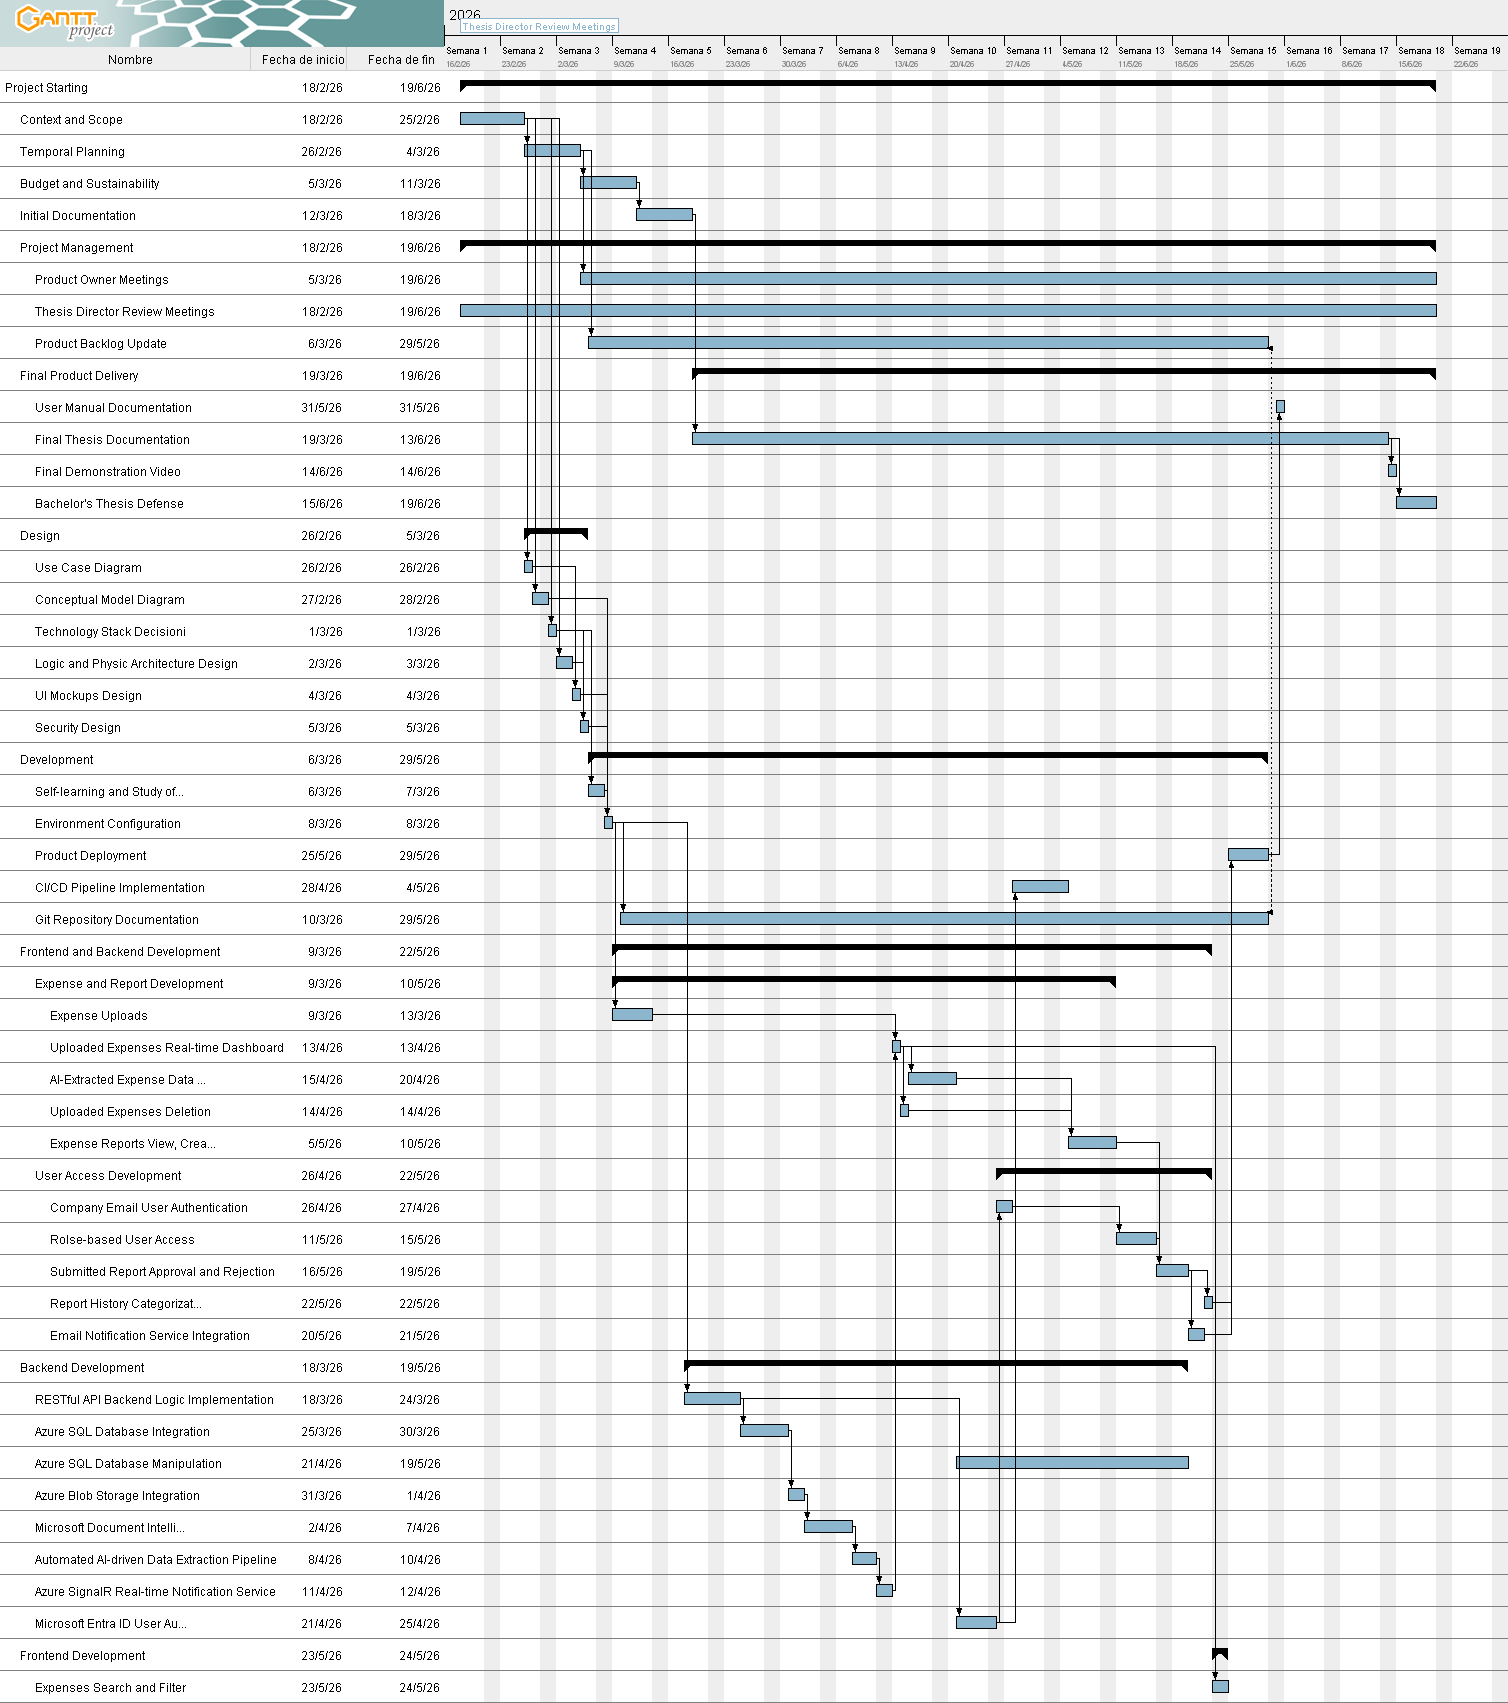
\includegraphics[width=\textwidth]{Images/Gantt2.png}
    \caption[Actual project Gantt diagram]
    {Actual project Gantt diagram. [Own creation]} 
    \label{fig:gantt2} 
\end{figure}   

 Before diving into the details of the deviations between the planned and actual project execution, note that a minor adjustment was made to the \textbf{UA5} task. The original task name, “Submitted and Reviewed Expenses Records Visualization,” was replaced with the more descriptive name “Report History Categorization by Status and User Role.” 

The \textbf{UA5} task was renamed because it was upgraded by the Product Owner during project execution. A more accurate description is that it involves developing a dashboard for each report status: for employees, dashboards showing “Not Sent” and “Submitted” reports, and for admins, dashboards showing “Pending Review” and “Reviewed” reports.

Looking at Table \ref{table:comparison-of-planned-and-actual-effort-per-task}, the project clearly overspent its schedule: the initial plan was \textbf{513 hours}, but the actual effort reached \textbf{542.5 hours}. However, as shown in the Gantt diagram in Figure \ref{fig:gantt2}, the project was still executed within the planned \textbf{122 days}.

Comparing each task's planned time with its actual effort shows that some tasks exceeded their estimates while others required less time. The most significant underestimation occurred in task \textbf{FPD2} (final thesis documentation), which overran by 49.5 hours. The author acknowledges this clear underestimation of effort.

Other overrunning tasks were \textbf{Dev2} (product deployment), \textbf{UA3} (submitted report approval and rejection), and \textbf{BD2} (Azure SQL database integration and manipulation). These tasks required more effort than initially calculated. The root cause of this underestimation is the author's inexperience with database manipulation and product release.

Several tasks, however, were completed faster than expected: \textbf{Dev5}, \textbf{UA6}, \textbf{BD4}, and \textbf{BD5}. \textbf{Dev5} involved creating clear repository documentation to help future developers understand the project context. The originally estimated 40 hours were reduced by half. 

\textbf{UA6}, \textbf{BD4}, and \textbf{BD5} tasks involved Azure resources. The initial approximation included a buffer because this was the author's first experience with cloud platforms. However, Azure Portal's intuitive interface and the straightforward handling of Azure resources through the .NET platform enabled efficient execution of these tasks.

Despite the time gained on some tasks, the overruns on others were larger, so the total execution time still exceeded the established effort. As explained in Section \ref{sec:temporal-planning}, this bachelor's thesis is organized for 540 total hours; the 27-hour buffer is insufficient, and actual execution has already surpassed the planned workload. To keep the project within budget, some tasks were discarded following the MoSCoW approach.

Tasks \textbf{UA4} and \textbf{FD2} are \textit{Could have} functionalities with low priority. Omitting them does not significantly impact the final product value, so they are not included in the actual Gantt diagram. Another missing task in the Gantt diagram is \textbf{Dev4}, which involves logging and monitoring the application. It is also low-priority, and omitting it does not affect the product's final value.

During project execution, dedicating one week to \textbf{Dev3} task (CI/CD Pipeline Implementation) revealed a shortfall compared to the original approximation of five days due to the author's lack of expertise. The execution was already exceeding the planned allocation, the task is not high-priority and has no strong dependencies on other tasks.

Given these circumstances, \textbf{Dev3} was rescheduled to the final development stage and ultimately discarded. By the project's final stage, no buffer time remained for its completion, leaving the possibility to implement this task in future iterations.

Despite all the challenges encountered and the incomplete execution of the project, the final product fulfills all high-priority and medium-priority requirements (\textit{Must have} and \textit{Should have}) thanks to the MoSCoW strategy. As a result, an application that delivers optimal value within the timeline, as well as within the author's capabilities and expertise, has been delivered.
